\documentclass[../Livrable1.tex]{subfiles}
\usepackage{hyperref}
\usepackage{array}

\begin{document}

\title{Architecture Réseau et Plan d’Adressage IP}
\author{}
\date{}
\maketitle

\section*{Architecture Réseau}

Nos objectifs pour ce projet sont de \textbf{concevoir} et \textbf{mettre en œuvre} une \textbf{infrastructure de réseau} qui soit capable d’accueillir les postes de travail des utilisateurs d’une organisation en apportant à ces utilisateurs un certain nombre de services.

Cette \textbf{infrastructure devra être sécurisée} : on cherche à protéger les machines, les réseaux et les données de cette organisation contre les cybermenaces courantes.  
Pour remplir ces objectifs, nous avons imaginé une architecture réseau en plusieurs sous-réseaux :

\begin{itemize}
    \item \textbf{Utilisateurs} : ce sous-réseau sert à contenir les postes utilisateurs.
    \item \textbf{Administrateurs} : le sous-réseau administrateur donne un accès privilégié à tous les réseaux de l’entreprise, il sert aussi à stocker des données administrateurs.
    \item \textbf{Serveurs internes} : pour les bases de données, applications internes, etc.
    \item \textbf{DMZ} : la DMZ contient les sites web publics.
\end{itemize}

Nous mettrons aussi en place un \textbf{serveur de fichiers} pour les postes de travail.

Pour \textbf{relier notre réseau à Internet}, nous devons mettre en place un \textbf{routeur}. Pour \textbf{sécu\-ri\-ser ce routeur}, nous ajouterons un \textbf{pare-feu} pour filtrer les entrées et sorties réseau.

La communication avec Internet nécessite une adresse IP ; nous les attribuerons \textbf{dyna\-mi\-quement} avec un \textbf{serveur DHCP} par sous-réseau afin de ne pas surcharger un DHCP central.

Enfin, nous devons résoudre les URLs en adresses IP grâce à un \textbf{serveur DNS}, le premier sera \textbf{interne} pour résoudre les \textbf{adresses des sous-réseaux} non accessibles depuis l’extérieur, et le deuxième \textbf{externe} pour résoudre les \textbf{adresses en ligne}.

Cette architecture nous donne le schema suivant : 
\begin{figure}[h]
    \centering
    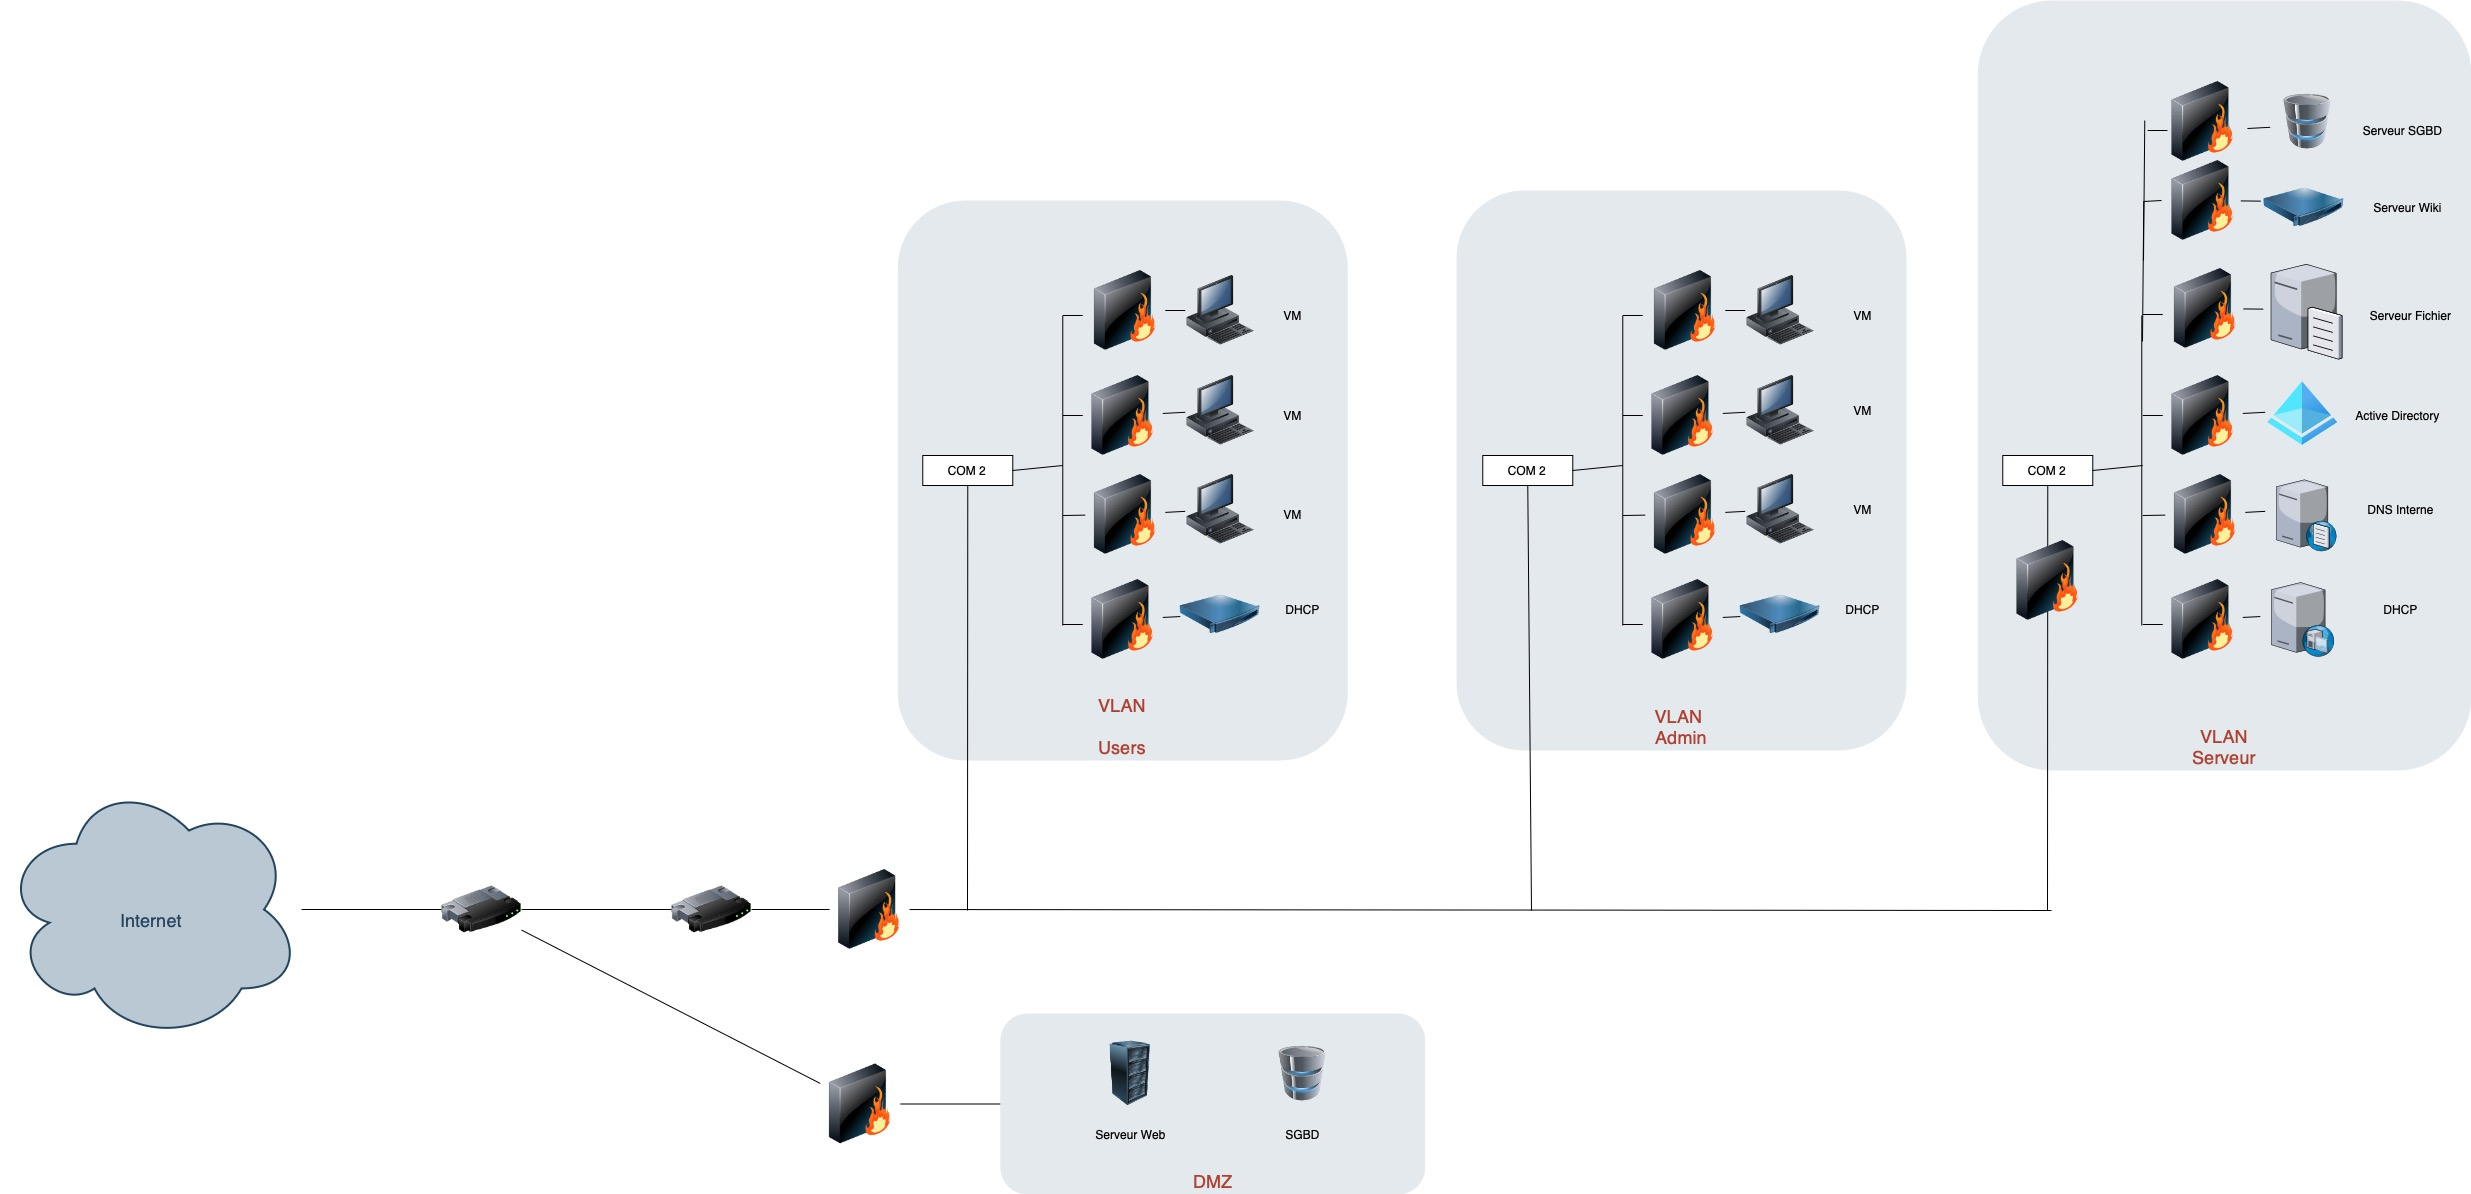
\includegraphics[width=0.7\textwidth]{../images/Architecture.jpg}
    \caption{Schema de l'architecture réseau}
    \label{fig:architecture}
\end{figure}

\section*{Plan d’Adressage IP}

Pour un plan d’adressage IP, on choisit une \textbf{plage privée (RFC1918)}, ici \texttt{10.X.X.0/24}, puis nous attribuons ensuite les adresses des sous-réseaux et des machines :

\begin{table}[h]
    \centering
    \begin{tabular}{|l|c|c|}
        \hline
        \textbf{Sous-Réseau} & \textbf{Adresse IP} & \textbf{Masque} \\
        \hline
        Routeur & 10.0.1.1 & 255.255.255.0 \\
        Réseau Utilisateurs & 10.0.10.0 & 255.255.255.0 \\
        Réseau Admins & 10.0.20.0 & 255.255.255.0 \\
        Réseau Serveurs & 10.0.30.0 & 255.255.255.0 \\
        DMZ & 10.0.40.0 & 255.255.255.0 \\
        DHCP Server & 10.0.30.10 & 255.255.255.0 \\
        DNS Interne & 10.0.30.20 & 255.255.255.0 \\
        DNS Externe & 10.0.40.20 & 255.255.255.0 \\
        Pare-feu & 10.0.1.254 & 255.255.255.0 \\
        \hline
    \end{tabular}
    \caption{Plan d’adressage IP}
\end{table}

On notera que tous les postes clients \textbf{reçoivent leurs IPs via DHCP} et que les serveurs ont des \textbf{adresses IP statiques}.
\end{document}